\section{Domain Name System}

\subsection{Fundamentals}
Host names are mnemonic names that can be easily memorized by humans and have variable length, yet provide little information about the location. Therefore, the Domain Name System provides the translation from a host name to an IP address. For example, it can translate \texttt{www.google.com} to \texttt{216.58.200.4}. It can also provide additional information. 

DNS is a performance-critical distributed database, which heavily leverages caches at different levels, allowing faster lookup. DNS security is critical for the web since the Same-Origin Policy assumes that DNS is secure; otherwise, a user might be redirected to a wrong or even malicious server. 

\begin{minipage}{0.34\textwidth}
DNS is a hierarchical decentralized naming system, i.e., the host name space is divided into zones. DNS consists of a hierarchy of distributed name servers, including:\\[3pt]

- root servers for top-level domains (TLD)\\[3pt]

This is hardcoded into other servers.\\[3pt]

- authoritative name servers for subdomains\\[3pt]

- local name resolvers\\[3pt]
\end{minipage}
\begin{minipage}{0.65\textwidth}
  \begin{figure}[H]
    \centering
    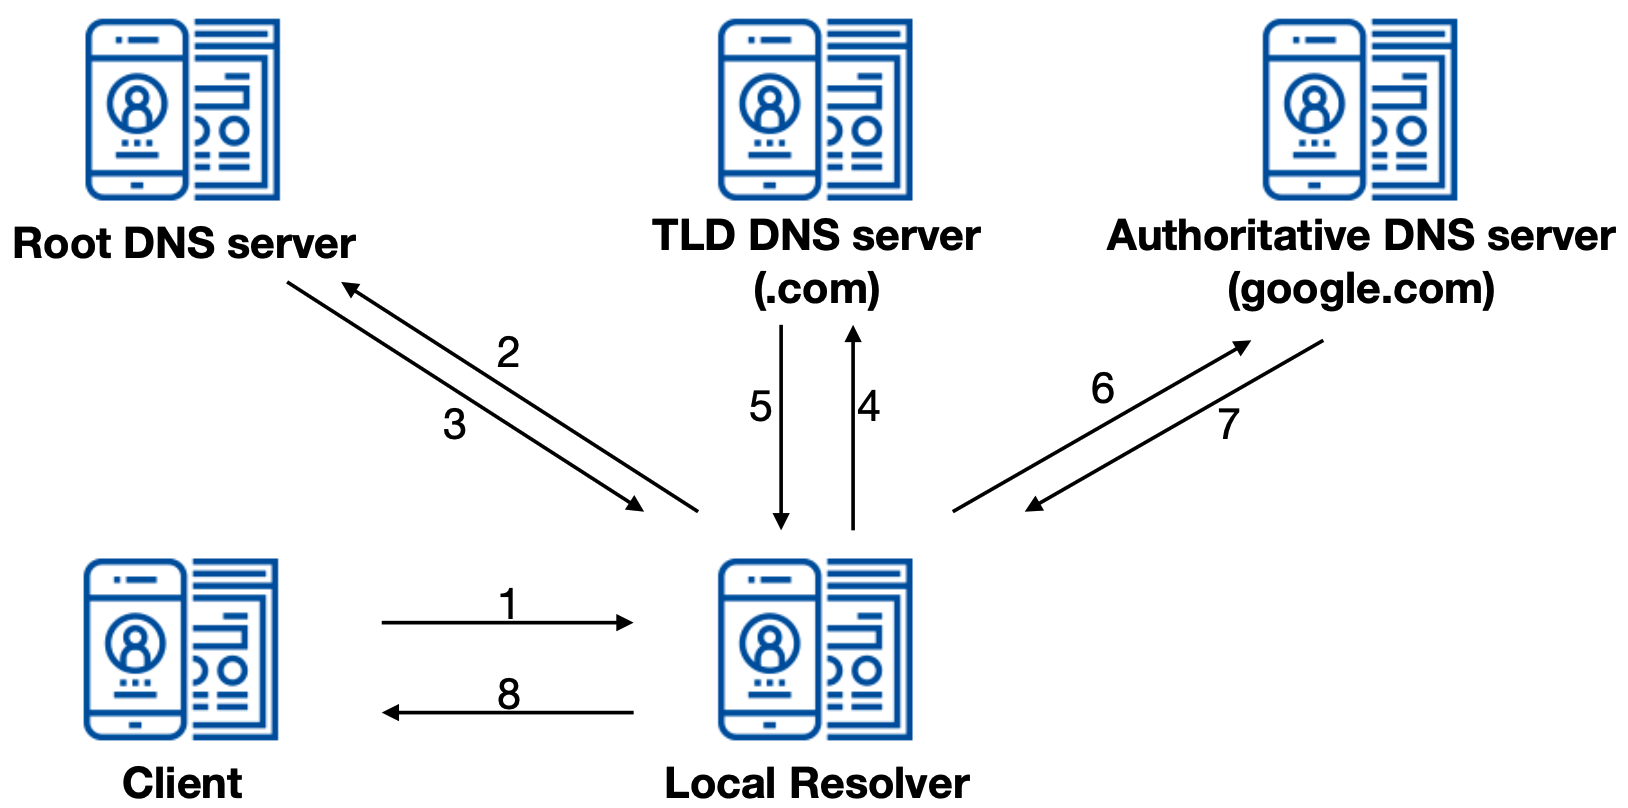
\includegraphics[width=\textwidth]{Figure/DNSLookup.png}
    \caption{DNS Lookup}
  \end{figure}
\end{minipage}

This caches name resolution results and asks authoritative name servers for unknown names.

A DNS packet is structured like the following: 

\begin{figure}[H]
  \centering
  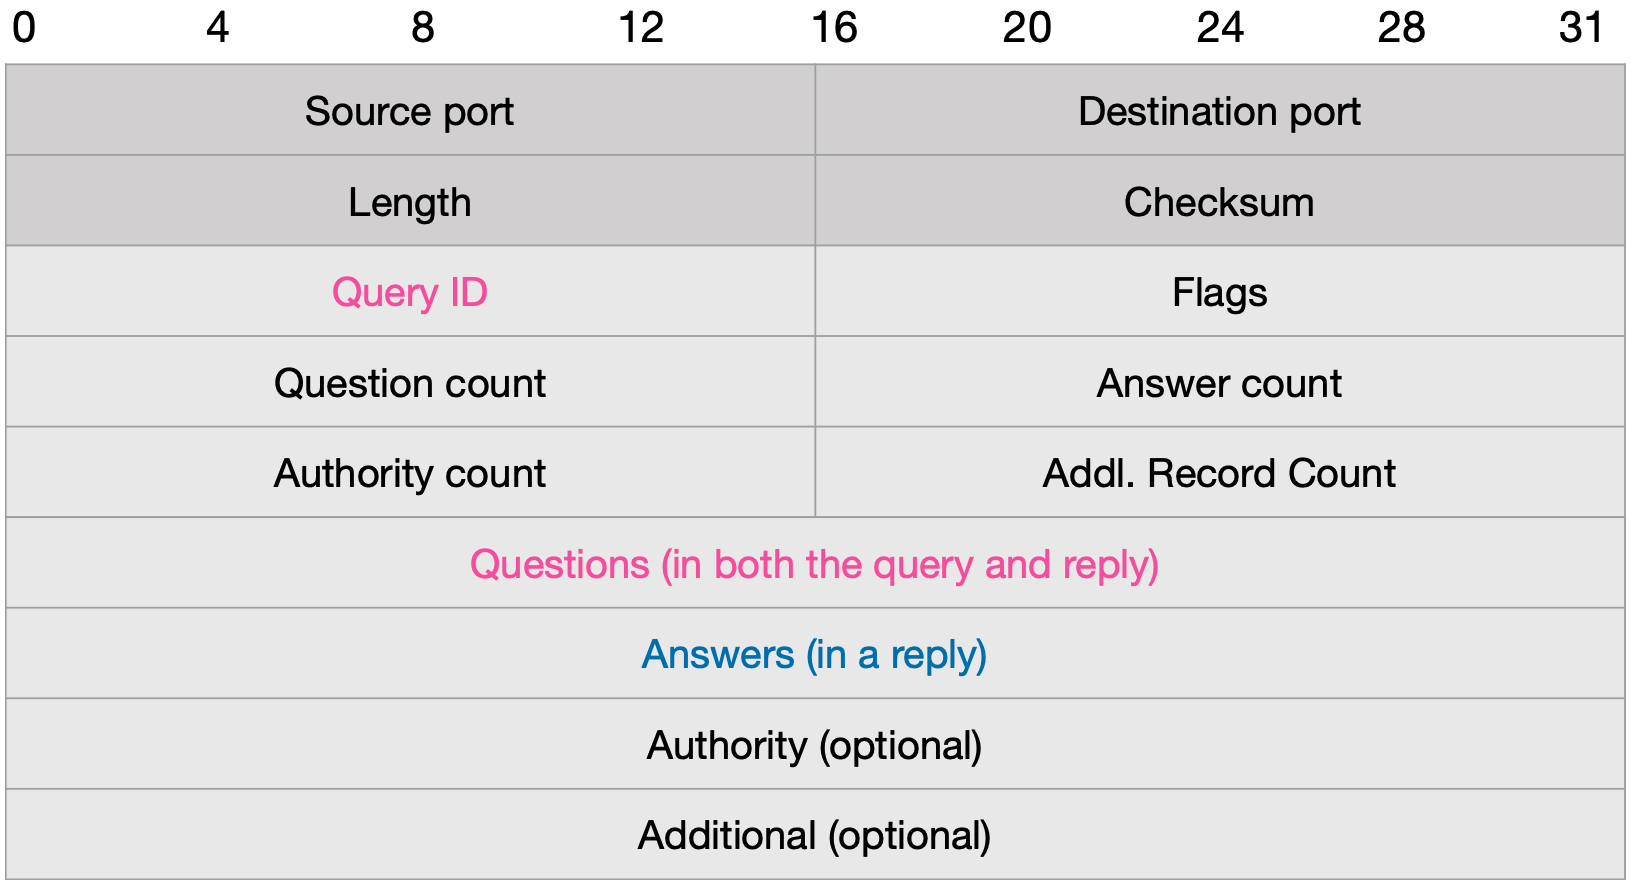
\includegraphics[width=0.7\textwidth]{Figure/DNSPacket.png}
  \caption{DNS Packet}
\end{figure}

\subsection{DNS Resource Records}
DNS resources have different types, including:

- Address Mapping records (A)  

This maps a host name to an IP address.  

- Canonical Name records (CNAME)  

This points a host name to another name (alias).  

- Mail Exchange records (MX)  

Directs email to a particular mail server.  

- Name Server records (NS)  

Specifies an authoritative name server for the given domain.  

- Start of Authority records (SOA)  

This specifies core information about a DNS zone, including the primary name server and the email of the domain administrator.  

\subsection{Caching}
Caching is extensively used in DNS to minimize lookups. It allows quick DNS responses for repeated translations. For DNS negative queries, it also caches non-existing domains to save time for future queries of non-existing host names.  

Cached data will periodically time out. Time To Live (TTL) is controlled by the owner of the data and is included with every record. 

\subsection{Threats}
DNS is sent over UDP; thus the identification number and ports are the only information used for ``security''. DNS has no confidentiality, authentication, or integrity guarantees. Therefore, an attacker is able to learn which hosts a victim communicates with by eavesdropping on DNS queries. They can also control a victim's traffic by poisoning the DNS cache. 

For example, we have a DNS query as follows:

\begin{verbatim}
; <<>> DiG 9.10.6 <<>> A www.cse.cuhk.edu.hk
;; global options: +cmd
;; Got answer:
;; ->>HEADER<<- opcode: QUERY, status: NOERROR, id: 58997
;; flags: qr rd ra; QUERY: 1, ANSWER: 2, AUTHORITY: 4, ADDITIONAL: 5

;; QUESTION SECTION:
;www.cse.cuhk.edu.hk. IN A

;; ANSWER SECTION:
www.cse.cuhk.edu.hk. 1747 IN CNAME fortress.cse.cuhk.edu.hk.
fortress.cse.cuhk.edu.hk. 1748 IN A 137.189.91.192

;; AUTHORITY SECTION:
cse.cuhk.edu.hk. 3025 IN NS garden.cse.cuhk.edu.hk.
cse.cuhk.edu.hk. 3025 IN NS beryl.cse.cuhk.edu.hk.
cse.cuhk.edu.hk. 3025 IN NS sapphire.cse.cuhk.edu.hk.
cse.cuhk.edu.hk. 3025 IN NS cucs18.cse.cuhk.edu.hk.

;; ADDITIONAL SECTION:
beryl.cse.cuhk.edu.hk. 3025 IN A 137.189.91.187
cucs18.cse.cuhk.edu.hk. 3025 IN A 137.189.91.190
garden.cse.cuhk.edu.hk. 3025 IN A 137.189.91.188
sapphire.cse.cuhk.edu.hk. 3025 IN A 137.189.91.189
\end{verbatim}

Here, the question section includes the query the client requested. Each query or reply has an ID, which is a 16-bit transaction identifier. This allows the DNS client to match the reply with the query. 

The answer section includes a resource record (RR), which tells the client the IP address of the domain name it asked for, as well as how long it should cache the answer. 

The authority section tells the name servers that are responsible for the answer. Each RR gives the hostname of a different name server. The client would send the query to one of these name servers if the answer section is empty. 

The additional section provides additional information that the client may find useful, e.g., an RR can provide the IP address of a hostname returned in the authority section. 

\subsubsection{Malicious DNS Server}
If the user connects to a malicious DNS server, it can fool the user about the answer to the DNS query. It can also provide the IP address of a host controlled by the attacker as the answer. A malicious DNS server can also be used to poison cache entries and mislead users about other queries. 

Then a malicious record could become:

\begin{verbatim}
;; AUTHORITY SECTION:
cse.cuhk.edu.hk. 3025 IN NS garden.cse.cuhk.edu.hk.
cse.cuhk.edu.hk. 3025 IN NS beryl.cse.cuhk.edu.hk.
cse.cuhk.edu.hk. 3025 IN NS sapphire.cse.cuhk.edu.hk.
cse.cuhk.edu.hk. 3025 IN NS www.abc.edu.hk.

;; ADDITIONAL SECTION:
beryl.cse.cuhk.edu.hk. 3025 IN A 137.189.91.187
www.abc.edu.hk. 3025 IN A 137.189.91.190
garden.cse.cuhk.edu.hk. 3025 IN A 137.189.91.188
sapphire.cse.cuhk.edu.hk. 3025 IN A 137.189.91.189
\end{verbatim}

To fix such issues, the client should not accept a record in the additional section if the record is not relevant to the domain being queried, i.e., deny records for unrelated domains. 

\subsubsection{Eavesdropping}
If an on-path attacker can eavesdrop on traffic, they can easily control or observe Internet traffic. For an off-path attacker, they can still attack by performing spoofing attacks. 

Since an on-path attacker can see the 16-bit transaction ID in the query, they can spoof a reply and race against the real DNS server response. This is also one way to perform censorship. 

\textbf{Blind Spoofing} 

An off-path attacker tries to inject a forged reply into a local resolver's cache, which can poison multiple hosts using the additional field. However, the attacker needs to know the ID and the port. The port is normally 53, and the challenge is that the attacker must guess the transaction ID. 

To guess the ID, it can be done randomly. However, since the ID is often incremented sequentially, the attacker can trick the victim into submitting a DNS lookup query to a DNS server controlled by the attacker. This can be mitigated by using random IDs, but attacks are still possible. 

\textbf{Kaminsky Blind Spoofing}

To guess the ID, the attacker tricks the victim into submitting many queries. Then they inject many forged replies with different IDs. This can be done by sending queries for many non-existing hostnames, causing the resolver to generate many queries with different IDs. The attacker succeeds if any forged response matches a valid ID. 

To defend against this, since the ID field is only 16-bit, we increase entropy by using a random source port in the query. We can also send multiple queries with different IDs, but this increases DNS load. However, not all resolvers have implemented random source ports.

\subsection{DNSSEC}
The DNS Security Extensions provide \textbf{origin authentication} and \textbf{integrity assurance}. 

At each level of the DNS lookup, DNS data is signed by the private key of the DNS server, and its public key is vouched for by the upper-layer server. The root DNS server's public key is hardcoded, forming a chain of trust. The signed keys and signed DNS data can also be cached. 

For DNSSEC, the DNS packet header is not changed; instead, authentication and integrity data are added as new resource records, including:

- RRSIG: signature of a resource record set (RRset) using the private key of a zone  

- DNSKEY: public key of a zone  

- DS: cryptographic digest of the public key of a child zone  

- NSEC / NSEC3: authenticated denial of existence  

The raw DNS records are not directly trusted; instead, their authenticity is verified through a signed chain of trust. At each step: the parent provides a DS record, the child provides a DNSKEY, the resolver matches them, and then trusts the child zone.  

For example, when a local host wants to resolve \texttt{www.google.com}, it sends a query to the local resolver, which performs a recursive lookup starting from the root DNS server. The root server responds with the name server for \textbf{.com}, along with a DS record and its signature, allowing the resolver to verify the \textbf{.com} key using the trusted root key.  

The resolver then queries the \textbf{.com} DNS server, which returns the name server for \texttt{google.com}, together with a DS record for \texttt{google.com}, signed by the \textbf{.com} key.  

Next, the resolver queries the authoritative DNS server for \texttt{google.com}, which provides the IP address along with a signature (RRSIG) and its public key (DNSKEY).  

The resolver verifies the chain of trust by first validating the \textbf{.com} key using the root key, then validating the \texttt{google.com} key using the DS record from \textbf{.com}, and finally using the verified \texttt{google.com} key to check the signature on the DNS record. Only if all these checks succeed will the resolver return the IP address to the client, ensuring the response is authentic and has not been tampered with.  

Note that the public key of a zone is returned in DNSKEY records. There are two types:

- Key Signing Key (KSK):  

Used to sign the DNSKEY records in the zone.  

- Zone Signing Key (ZSK):  

Used to sign other resource records (RRsets) in the zone.  

Separating the Zone Signing Key and Key Signing Key allows easier replacement of (compromised) ZSKs, since only the KSK needs to be signed by the parent zone.

\begin{figure}[H]
  \centering
  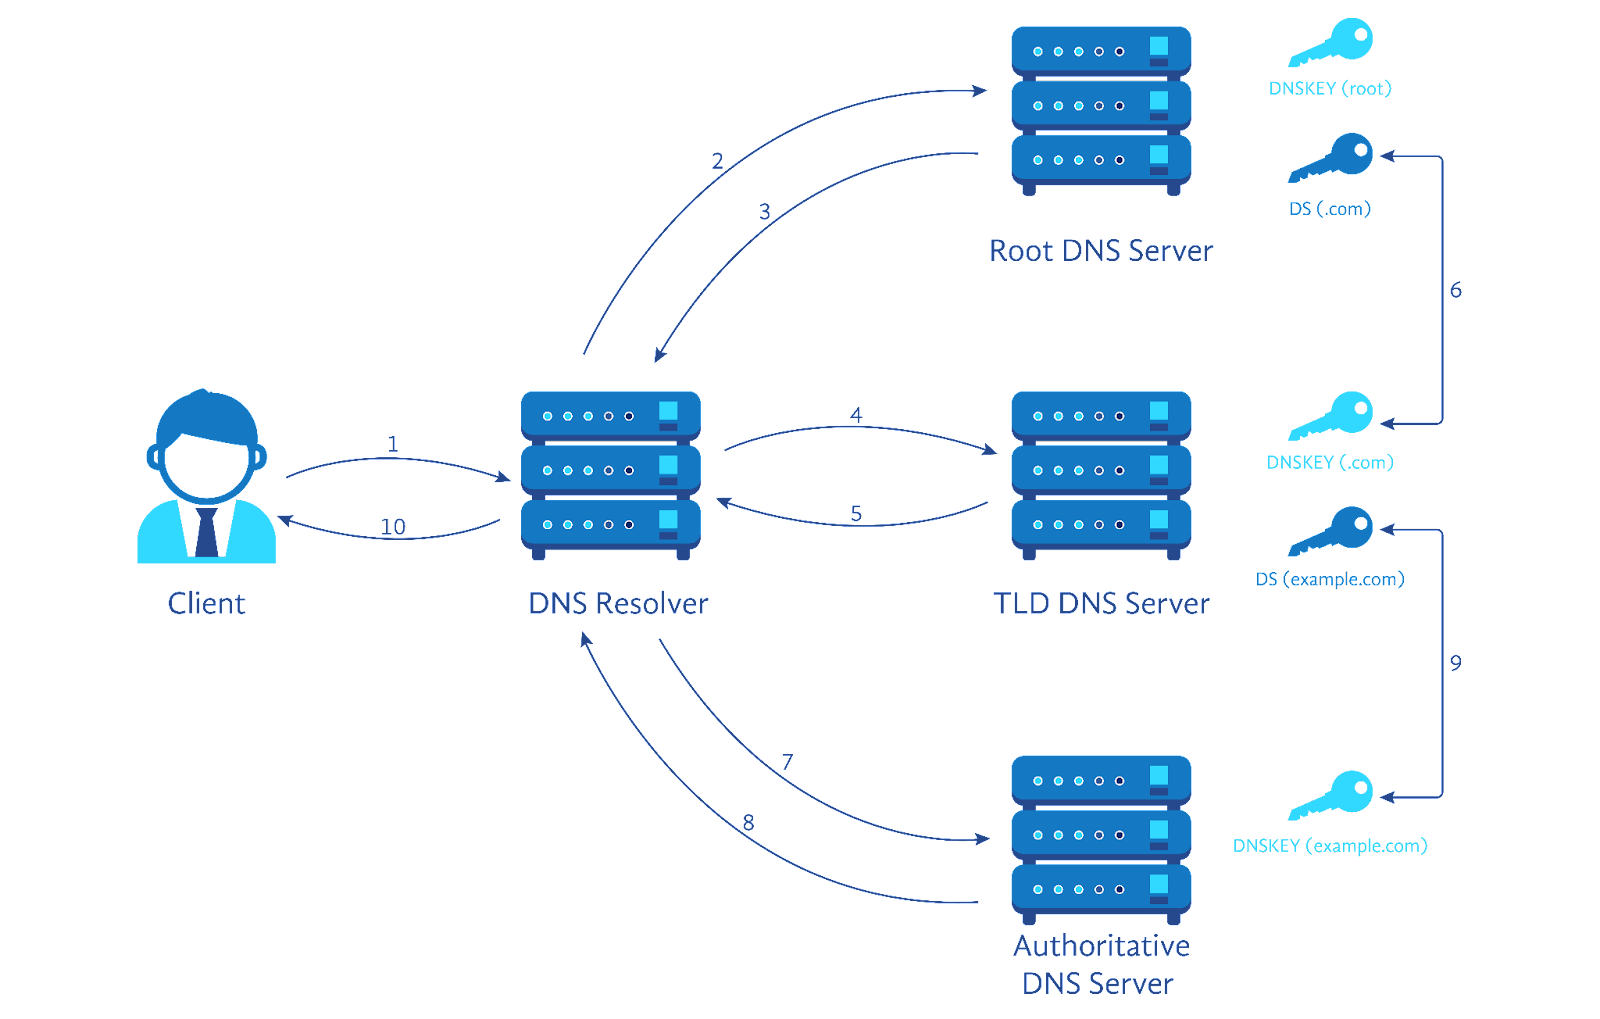
\includegraphics[width=0.7\textwidth]{Figure/DNSSEC.png}
  \caption{DNSSEC Lookup}
\end{figure}